\documentclass[11pt]{article}

% Packages
\usepackage[utf8]{inputenc}
\usepackage{amsmath, amssymb}
\usepackage{tcolorbox}
\usepackage{hyperref}
\usepackage{geometry}
\geometry{margin=1in}
\setlength{\parskip}{0.5em}

% Title
\title{Lecture 22: Unsupervised Pretraining of LLMs}
\author{STAT 479: Probabilistic Graphical Models\\Lecturer: Ben Lengerich\\Authors: Josh Salinas and Mitchell Stephens}
\date{April 17, 2025}

\begin{document}

\maketitle

\section*{Announcements}
\begin{itemize}
    \item Project presentations: April 29 and May 1.
    \item Submit peer review forms on Canvas each day to earn up to 2\% bonus.
    \item Due by: Friday, May 2.
\end{itemize}

\section{Unsupervised Training of LLMs}
\subsection*{Maximum Likelihood Estimation (MLE)}
\begin{itemize}
    \item GPT models maximize the likelihood of observed sequences:
    \[ \max_{\theta} \sum_{i=1}^T \log P_{\theta}(x_i \mid x_{<i}) \]
    \item This is a Directed Probabilistic Graphical Model.
    \item Predicting even simple tokens (e.g., "is" in a factual sentence) requires grammar, factual knowledge, and context resolution.
    \item Positional encodings are added to input embeddings to provide sequence order information.
\end{itemize}

\subsection*{Historical Context}
\begin{itemize}
    \item MLE-based models have existed since 2007.
    \item 2007 google MLE-base language model had 2 trillion tokens and 300 billion n-grams
    \item Early models focused on n-grams, not embeddings.
    \item Lack of deep representation and contextual modeling.
    \item The LLM breakthrough came with transformers, large datasets, and GPU acceleration.
\end{itemize}
\subsection*{GPU Importance}
\begin{itemize}
    \item CPUs have less cores typically between 4-8
    \item Each core has an L1 and Control which allow for more difficult computation
    \item GPUs can split cores to make hundreds which allow for more basic tasks to be completed faster like matrix multiplication
    \item The only downfall to this is there is no interaction between cores and takes longer to access data from memory but overall allow for quicker computation
    
    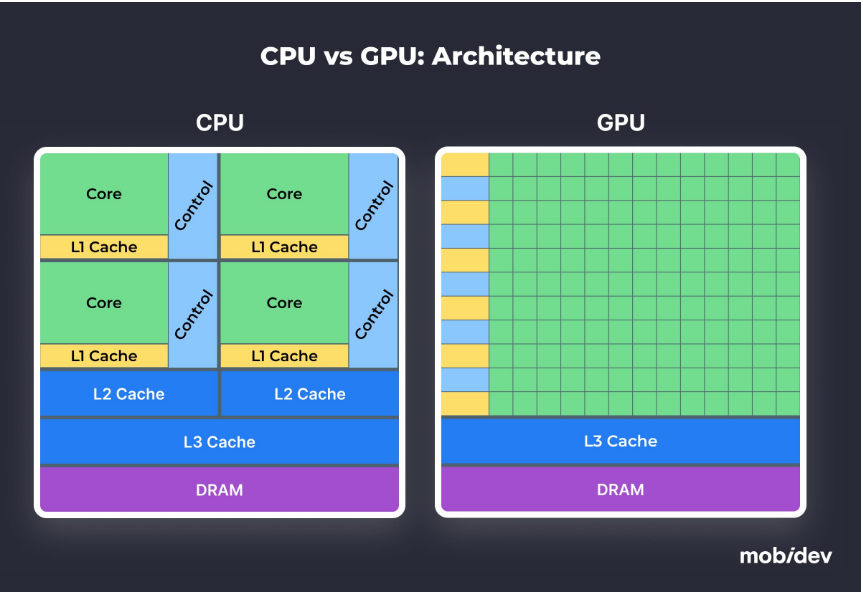
\includegraphics[width=0.8\textwidth]{notesimage1.PNG}
\end{itemize}

\section{Scale and Emergent Capabilities}
\begin{itemize}
    \item As model scale increases, new capabilities emerge unexpectedly.
    \item Examples: in-context learning, chain-of-thought reasoning.
    \item Refer to: \textit{Scaling Laws for Neural Language Models} (Kaplan et al. 2021).
\end{itemize}

\begin{tcolorbox}
\textbf{Example:} Predicting ``is'' in ``The capital of France \_\_ Paris'' requires
\begin{itemize}
    \item Subject-verb agreement
    \item Recognition of factual structures
    \item Geographical knowledge
\end{itemize}
\end{tcolorbox}

\subsection*{In-Context Learning}
\begin{itemize}
    \item Once you train a few models the model will learn quickly on how to apply P(x)
    \item Zero Shot the model is only given instructions with no examples
    \item Few-Shot with instruction the task is given along with examples and instructions
    \item Few-Shot with only examples no instruction is given the model must infer from the examples provided
    
    
    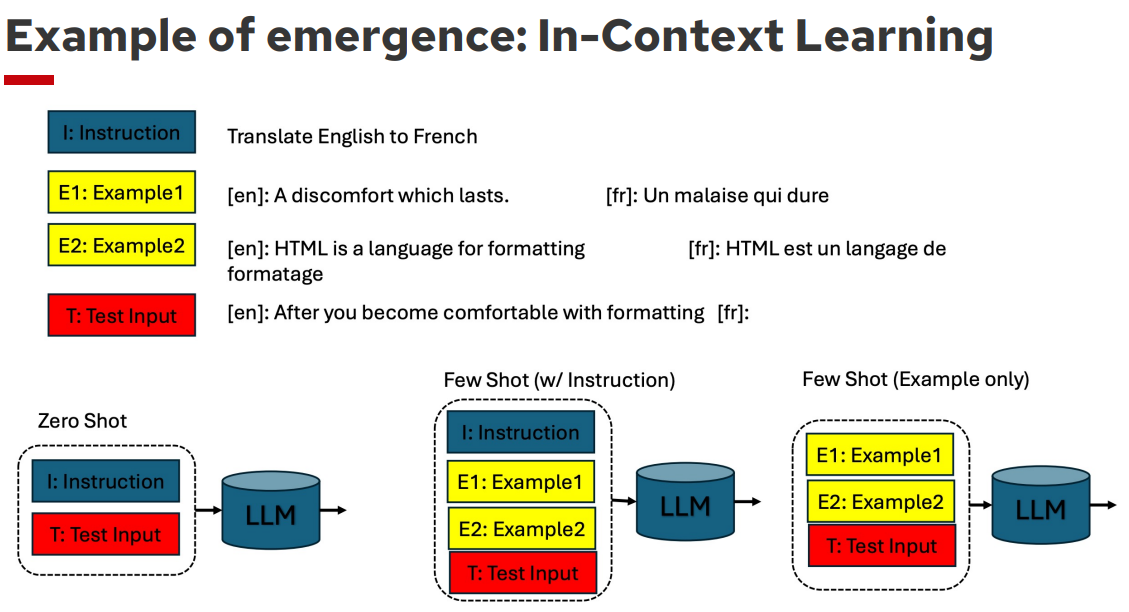
\includegraphics[width=0.9\textwidth]{notesimage2.PNG}
\end{itemize}

\subsection*{Chain-of-Thought}
\begin{itemize}
    \item Chain-of-Thought is asking the model to explain its work and reasoning
    \item An example would be showing all steps of solving a derivative of a complex equation
    \item Showing the correct reasoning will help the model adapt quickly and provide more accurate responses
    \item This leads to better performance especially on more complex tasks and problems
\end{itemize}

\subsection*{Why Does This Work?}
\begin{itemize}
    \item No proven reason on how or why this works
    \item Some hypothesis are task identification is implicit Bayesian inference
    \item Transformers learn in-context by using gradient descent
    \item Could also be a mix of both
\end{itemize}

\subsection*{Scale}
\begin{itemize}
    \item Scale adds more randomness and diversity
    \item It does not just overfit the data due to all the arbitrary models will cancel each other out which leads to the ensemble being a good model.
    \item As you increase parameters you also increase variance
    \item More randomization is good for more hyper-specific individual models
    \item However this can be difficult for data filtering and preparation
    \item Fitting to bad data will lead to a bad distribution which will make the model worse
    
    
    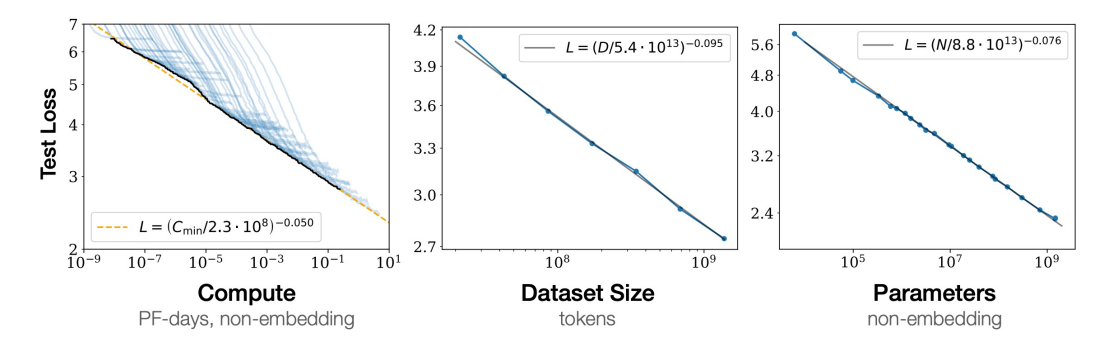
\includegraphics[width=0.9\textwidth]{notesimage3.PNG}
\end{itemize}

\section{Challenges of MLE}
\subsection*{KL Divergence Minimization}
\begin{itemize}
    \item MLE objective: \[ \arg\max_{\theta} \mathbb{E}_{x \sim P_{\text{data}}}[\log P_{\theta}(x)] = \arg\min_{\theta} \text{KL}(P_{\text{data}} \| P_{\theta}) \]
    \item Issues:
    \begin{itemize}
        \item Repetitiveness, memorization of training data
        \item Lack of semantic grounding or task objectives
        \item Must assign probability to all plausible sequences, including incoherent ones
        \item MLE is not task-aware — it doesn't optimize for downstream accuracy or meaning
    \end{itemize}
\end{itemize}

\subsection*{Entropy and Confidence}
\begin{itemize}
    \item Token-level entropy:
    \[ H_t = -\sum_v P(x_t = v \mid x_{<t}) \log P(x_t = v \mid x_{<t}) \]
    \item Lower entropy = higher model confidence.
    \item Only want this if there is confidence the model has learned well and the output will be correct
    \item Models may output overly generic or repetitive text when entropy is low.
    \item Sampling strategies (e.g., greedy, top-k, nucleus sampling) help control generation diversity.
\end{itemize}

\section{Links to Variational Inference}
\begin{itemize}
    \item ELBO:
    \[ \log p(x \mid \theta) \geq \mathbb{E}_{z \sim q}[\log p(x,z \mid \theta)] + H(q) \]
    \item Maximizing ELBO encourages higher entropy in latent variables.
    \item MLE lacks explicit entropy control.
\end{itemize}

\section{Solutions to MLE Limitations}
\begin{itemize}
    \item Entropy regularization:
    \[ \theta^* = \arg\max_{\theta} \mathbb{E}_{x \sim P_{\text{data}}}[\log P_{\theta}(x)] + \lambda \cdot H[P_{\theta}(x)] \]
    \item Smooth labeling:
    \[ y'_i = \begin{cases} 1 - \epsilon & y = 1 \\ \epsilon / (V - 1) & y \neq 1 \end{cases} \]
    \item Other solutions discussed:
    \begin{itemize}
        \item Contrastive learning (e.g., noise contrastive estimation)
        \item Preference- or utility-based training (e.g., RLHF)
        \item Risk minimization (optimize for downstream task loss rather than log-likelihood)
        \item Scheduled sampling
        \item Objectives for coverage and diversity
        \item Adding a penalty for low entropy
    \end{itemize}
\end{itemize}

\section*{References and Tools}
\begin{itemize}
    \item Radford et al., \textit{Improving Language Understanding by Generative Pre-Training}
    \item Holtzman et al., \textit{The Curious Case of Neural Text Degeneration}
    \item Hugging Face TxT360: \url{https://huggingface.co/spaces/LLM360/TxT360}
    \item https://mobidev.biz/blog/gpu-machine-learning-on-premises-vs-cloud
    \item Kaplan et al 2021., \textit{Scaling Laws for Neural Language Models}
\end{itemize}

\end{document}
